\documentclass[addpoints]{exam}
\usepackage{url}
\usepackage{amsmath,amsthm,enumitem}
\usepackage{graphicx}
\usepackage{qtree}
\usepackage[nodayofweek,level]{datetime}
\usepackage{color}
\usepackage{csquotes}
\usepackage{pgf, tikz}
\usetikzlibrary{arrows, automata}
\usepackage{algorithm,algpseudocode}

\definecolor{qcolor}{rgb}{0, 0, 0.3}
\definecolor{acolor}{rgb}{0, 0, 0}

%\input myfonts

\lhead{Gopal Menon (u0772360)}
\chead{\bf{HW1}}
\rhead{CS 6150 \today}
\headrule

\begin{document}

\section*{Collaborators}

Ben Nelson and I collaborated for this assignment on all questions except question $2$. We discussed $5c$ in some detail and discussed the rest without going into too many specifics.
\qformat{Question \thequestion: \thequestiontitle\dotfill \textbf{[\totalpoints]}}\pointname{}\bonuspointname{}\pointformat{[\bfseries\thepoints]}
\begin{questions}

\color{qcolor}
\titledquestion{Prefix trees revisited}[8]
Recall the prefix tree data structure for storing a collection of strings (Lecture 2). Suppose we wish to support the following operations: ADD string, DELETE string, QUERY string, COUNT-PREFIX. The last operation takes a string $w$ and returns the number of strings in our collection having $w$ as a prefix.

We saw how to build a data structure that supports the first three operations in time $O(|w|)$, where $|w|$ is the length of the string $w$ being added/deleted/queried. Describe a way to modify the procedures so that COUNT-PREFIX can also be answered in time $O(|w|)$.

\color{acolor}
A prefix tree is shown below with the strings $BED, PET, PAT, PATRON$ and $PATENT$. The root of the tree is denoted by $\circ$. Each node of the tree stores a letter that is part of a string along with a count that denotes the number of strings the letter is used in, a marker $\bullet$ when a string ends with the letter and an optional set of pointers to other nodes. A node can have an edge connecting it to another node when the two letters in the nodes are subsequent letters in a string. Although the tree shown does not have directional edges, the edges are to be read as if they were pointing downward. For example, the connected nodes $B, E $ and $D$ after the root show that the string $BED$ has been stored. Each of these letters have a count of $1$ to show that they have been used only in one string and the $\bullet$ after $D$ shows that the string $BED$ ends with the node $D$. The letter $P$ has a count of $4$ since it is used in strings $PET, PAT, PATRON$ and $PATENT$. There is a $\bullet$ marker on the letter $T$ in the middle of the string $PATENT$ since $PAT$ is also stored in the tree and the two strings have the first three letters common. 

\Tree[.$\circ$	[.B^1  [.E^1 [.D^1_{\bullet} ]]]
          		[.P^4 [.E^1 [.T^1_{\bullet} ]]
			      [.A^3 [.T^3_{\bullet} [.R^1 [.O^1 [.N^1_{\bullet} ]]]
			      		 [.E^1 [.N^1 [.T^1_{\bullet} ]] ]] ]]]
					 
\textbf{QUERY procedure algorithm:} For the QUERY operation, a client of the prefix tree will start at the root and look for connected nodes starting with the first letter of the string being queried and ending with the last letter of the string. If the last node also has a $\bullet$ marker, then it means that the string being queried, is present in the tree. So the string $BE$ will not be found in the tree even though nodes $B$ and $E$ exist after the root, but the string $BED$ will be found. 

\textbf{QUERY procedure correctness:} Consider the case where the string being queried does not exist in the tree. This could be because the string exists only as a prefix or does not exist at all. In the former case, although the entire query string is found in the tree, since the last letter of the query string will not have a $\bullet$ marker, the procedure will return a result of not found. In the latter case, the in order connected nodes corresponding to the query string will not be found in the tree and the procedure will return a result of not found. In the case the query string exists in the tree, there will be a set of connected nodes starting from the root that match with the string being queried and with the last node marked with a $\bullet$ marker. In this case the string being queried will be searched in the tree by looking for nodes starting after the root in the order of the letters in the query string and with the last node having a $\bullet$ marker. This will be found and the procedure will return a result of found.

\textbf{QUERY procedure running time:} This operation can be carried out in $O(|w|)$ time since the check can be done by navigating the tree starting at the root in order of the letters in the query string once.

\textbf{ADD procedure algorithm:} To ADD a string into the tree, the client will first $QUERY$ the string and if it is not found, start at the root and for a matching prefix of the string being added, that is already in the tree, it will increment the letter count. If the entire string is found, the last letter will be marked with a $\bullet$. If only a prefix of the string is found, the remaining letters will be added to the tree as connected nodes and letter count $1$ after the last letter of the prefix that was found. The last letter of the added string will be marked with a $\bullet$. The tree is shown below after the strings $BE$ and $BELL$ are added to the tree. 

\Tree[.$\circ$	[.B^2  [.E^2_{\bullet} [.D^1_{\bullet} ]]]
          		[.P^4 [.E^1 [.T^1_{\bullet} ]]
			      [.A^3 [.T^3_{\bullet} [.R^1 [.O^1 [.N^1_{\bullet} ]]]
			      		 [.E^1 [.N^1 [.T^1_{\bullet} ]] ]] ]]]

\Tree[.$\circ$	[.B^3  [.E^3_{\bullet} [.D^1_{\bullet} ]
				  [.L^1 [.L^1_{\bullet} ] ]]]
          		[.P^4 [.E^1 [.T^1_{\bullet} ]]
			      [.A^3 [.T^3_{\bullet} [.R^1 [.O^1 [.N^1_{\bullet} ]]]
			      		 [.E^1 [.N^1 [.T^1_{\bullet} ]] ]] ]]]
					 
\textbf{ADD procedure correctness:} Before a string is added to the tree, there is a check to see if it is already present in the tree. This prevents the string from being added to the tree again and keeps the letter usage counts correct and will ensure that the DELETE operation results in the string being removed from the tree if it is not being used as a prefix. For a prefix of a string being added, that is found in the tree, the letter counts are incremented by $1$. This will ensure that the COUNT-PREFIX operation returns the correct result. For a suffix of a string that is not found in the tree, a new branch will be started after the prefix that is found and connected nodes will be appended in order of the suffix with the last node having a $\bullet$ marker. This will ensure that a QUERY operation will find the string in the tree. If a prefix of the string being added is not found in the tree, connected nodes will be appended to the root node in order of the letters in the string being added. Each of these nodes will have a count of $1$ and the last node will be marked with a $\bullet$. This will ensure that a QUERY operation will find the string in the tree. If the string being added is found as a prefix in the tree, the letter usage counts will be incremented and the node corresponding to the last letter of the string will be marked with a $\bullet$. This will ensure that the COUNT-PREFIX and QUERY operations will return the correct result and the DELETE operation will not corrupt the tree after it decrements the letter counts. 

\textbf{ADD procedure running time:} An ADD operation as described above will take two operations (as a QUERY operation is called as part of the ADD) each with $O(|w|)$ checks and so the entire operation will take time $O(|w|)$.

\textbf{DELETE procedure algorithm:} To DELETE a string from the tree, the client will first QUERY the string and if it is found, start at the root and visit every node in order of the letters in the string. The count for each node will be decremented by $1$ and the $\bullet$ marker will be removed from the node corresponding to the last letter. At the point of decrementing the count, if it becomes $0$, the node will be removed. The tree is shown below after the strings $BED$ and $PAT$ are removed from the tree. 

\Tree[.$\circ$	[.B^2  [.E^2_{\bullet} 
				  [.L^1 [.L^1_{\bullet} ] ]]]
          		[.P^4 [.E^1 [.T^1_{\bullet} ]]
			      [.A^3 [.T^3_{\bullet} [.R^1 [.O^1 [.N^1_{\bullet} ]]]
			      		 [.E^1 [.N^1 [.T^1_{\bullet} ]] ]] ]]]

\Tree[.$\circ$	[.B^2  [.E^2_{\bullet} 
				  [.L^1 [.L^1_{\bullet} ] ]]]
          		[.P^3 [.E^1 [.T^1_{\bullet} ]]
			      [.A^2 [.T^2 [.R^1 [.O^1 [.N^1_{\bullet} ]]]
			      		 [.E^1 [.N^1 [.T^1_{\bullet} ]] ]] ]]]
					 
\textbf{DELETE procedure correctness:} Due to the count being decremented by $1$ as described above and and the $\bullet$ marker being removed from the node corresponding to the last letter, the COUNT-PREFIX operation will return the correct result and due to the nodes being removed when the decremented count reaches zero, a QUERY operation will return the correct result. Since a QUERY operation is performed before a string is removed through the DELETE operation, the case where a prefix of the string that exists and has usage counts decremented, but the string to be deleted does not exist in the tree, will not arise.

\textbf{DELETE procedure running time:} A DELETE operation will take two operations each with $O(|w|)$ checks and so the entire operation will take time $O(|w|)$.
					 
\textbf{COUNT-PREFIX procedure algorithm:} The COUNT-PREFIX operation will start at the root of the tree and visit every node in order of the letters in the string prefix. If it does not find a match for the prefix in the tree, it will return zero. If it finds the entire prefix in the tree, it will return the number associated with the last letter of the prefix in the tree. So in the example of the last tree shown above, a $COUNT-PREFIX$ operation with the prefix as $PA$ will return $2$. This means that the tree has two strings with $PA$ as the prefix. These strings are $PATRON$ and $PATENT$. 

\textbf{COUNT-PREFIX procedure correctness:} The ADD and DELETE procedures keep the letter counts updated correctly as described above. As a result of this, the COUNT-PREFIX returns the correct number. 

\textbf{COUNT-PREFIX procedure running time:} As the COUNT-PREFIX operation looks for a match of the prefix in the tree letter by letter, it can be completed in time $O(|w|)$.

\color{qcolor}
\titledquestion{Recurrences, recurrences}
Solve each of the recurrences below, and give the best $O(\cdot)$ bound you can for each of them. [{\em Hint: } You might find chapters 12 and 13 of the Lehman, Leighton book (available from the course homepage) useful.]

\begin{parts}
\part[3] $T(n) = 2T(\sqrt{n}) + 4$.
\part[4] $T(n) = T(n/3) + T(n/2) + \sqrt{n}$.
\part[5] Suppose you have devised a divide-and-conquer algorithm for a certain problem that breaks up a problem of size $n$ into three subproblems of size $n/2$ each, solves them recursively, and then combines the solutions. Suppose the time for breaking up and combination is given by $g(n)$. Suppose in your first attempt, you had a combine step that had $g(n) = n^{1.8}$. Does it make sense to think further and reduce $g(n)$ to $n^{1.5}$? What about reducing it even further to $g(n) = n \log n$? (Assume you only care about the asymptotic running time of the overall procedure.)
\end{parts}


\color{acolor}
\begin{parts}
\part \begin{equation*}
\begin{aligned}
T(n) &= 2T(\sqrt{n}) +4\\
&= 2T(n^{\frac{1}{2}}) +4\\
\text{Let }n &= 2^x \Rightarrow T(n) = T(2^x)\\
\text{Let }T(2^x) &= P(x)\\
P(x)&=2P \left (\frac{x}{2} \right ) + 4\\
&= 2P \left (\frac{x}{2} \right ) + O(1)\\
&= \Theta(\log(x))  \text{, using the Master Theorem \cite{CLRS} case 1, since $a=2$, $b=2$, $f(n) = O(1) = O(n^{log_b a-1})$}\\
P(x) &= \Theta(x)\\
&= \Theta(\log n))\\
\end{aligned}
\end{equation*}

\part \begin{equation*}
\begin{aligned}
T(n) &= T \left (\frac{n}{3} \right ) + T \left (\frac{n}{2} \right ) + \sqrt{n}\\
2T\left (\frac{n}{3} \right) + \sqrt{n} &\leq T(n) \leq 2T \left (\frac{n}{2} \right ) + \sqrt{n}
\end{aligned}
\end{equation*}
When we use the Master Theorem on the left inequality, $a=2$, $b=3$ and $f(n) = n^{0.5}$\\
$n^{log_b a} = n^{log_3 2}=n^{0.631}$\\
$f(n) = n^{0.5}=n^{log_b a -\epsilon}=O(n^{log_b a -\epsilon})$ for some $\epsilon > 0$\\
We can use case 1 of the Master Theorem, so\\
$T(n) \geq \Theta(n^{0.631})$\\
When we use the Master Theorem on the right inequality,\\
 $a=2$, $b=2$ and $f(n) = n^{0.5}=\Omega(n^{log_2 2 - \epsilon})=\Omega(n^{1 - \epsilon})$for some $\epsilon > 0$\\
We can use case 1 of the Master Theorem, so\\
$T(n) \leq \Theta(n)$\\
From the above two inequalities for $T(n)$, we can say that
\begin{equation*}
\begin{aligned}
T(n) &= \Theta(n^x) \text{, where } 0.631 \leq x \leq 1\\
\text{So }T(n) &= O(n) \text{ is the tightest upper bound I can find}
\end{aligned}
\end{equation*}

\part $T(n) = 3T(\frac{n}{2}) + g(n)$\\
For the first attempt $g(n) = n^{1.8}$\\
Using the Master Theorem, $a=3$, $b=2$, $log_b a = log_2 3 =1.585$\\
$f(n) = g(n) = n^{1.8} = \Omega(n^{1.8})=\Omega(n^{log_b a + \epsilon})$\\
$af(\frac{n}{b}) = 3\left ( \frac{n}{2} \right ) ^{1.8}=0.8615n^{1.8}$\\
$cf(n) = cn^{1.8}$\\
When $c=1$, $af(\frac{n}{b}) \leq cf(n)$\\
So by the Master Theorem, $T(n) = \Theta(n^{1.8})$\\

If we reduce $g(n)$ to $n^{1.5}$\\
$f(n) =  O(n^{1.5})=O(n^{log_b a - \epsilon})$\\
So by the Master Theorem, $T(n) = \Theta(n^{1.585})$\\
So it does make sense to reduce $g(n)$ to $n^{1.5}$\\

If we reduce $g(n)$ to $n \log n$\\
$g(n)= n\log n$ is upper bounded by $n^{log_b a} = n^{log_2 3} =n^{1.585}$, since $\log n$ is upper bounded by $n^{0.585}$.\\
So we can find an $\epsilon > 0$ such that $g(n) =O(n^{\log_b a-\epsilon})$.
So by case 1 of the Master Method, $T(n) = O(n{\log_b a}) = O(n^{1.585})$.
This does not give us an advantage over when $g(n)=n^{1.5}$.
\end{parts}

\color{qcolor}
\titledquestion{Bubble sort}
Recall the bubble sort algorithm (pseudocode at {\sf http://en.wikipedia.org/wiki/Bubble\_sort}). Recall that the worst case running time is $O(n^2)$.
\begin{parts}
\part[3] Give an example of an input array $A[]$ that is (a) not sorted to begin with, and (b) the algorithm takes time $O(n)$ on $A[]$.
\part[5] Give an example of an input array on which the algorithm takes time $\Theta(n^{3/2})$.
\end{parts}

\color{acolor}
\begin{parts}
\part Consider the case on an array where only the last element is out of place and everything else is sorted. Specifically, the last element is greater than the element two places before it, but less than the element just before it. The algorithm will scan the array from the beginning and will not swap any element till it comes to the last element. When it comes to the last element, it will swap it with the previous element. It will then scan the entire array except the last element, will not find anything to swap and will terminate. It will thus make two scans through the array and will take $O(2n)=O(n)$ time, where $n$ is the number of elements in the array. Consider the following example to illustrate this:
\begin{equation*}
\begin{aligned}
A &= \{21, 27,33,56,65,77,79,83,88,101,95\} \text{, is the initial state of the array}\\
A &= \{21, 27,33,56,65,77,79,83,88,95,101\} \text{, state of the array after last two elements have been swapped}\\
A &= \{21, 27,33,56,65,77,79,83,88,95,101\} \text{, unchanged state of the array after ino more swaps are needed}\\
\end{aligned}
\end{equation*}

\part Consider the case on an array with $n$ elements where the entire array except the last $\sqrt{n}$ elements are sorted and the last $\sqrt{n}$ elements are larger than then elements before them. The bubble sort algorithm will first scan the entire array and swap required elements in the last $\sqrt{n}$ part. Then it will scan the array up to the last but one element, then up to the last but two elements, and so on till element number $n-\sqrt{n}$. It will then stop. The number of elements scanned will be:
\begin{equation*}
\begin{aligned}
\text{Number of elements scanned} &= (\text{Sum of numbers $1$ through $n$}) -(\text{Sum of numbers $1$ though $n-\sqrt{n}$}) \\
&= \frac{n(n+1)}{2}-\frac{(n-\sqrt{n})(n-\sqrt{n}+1)}{2}\\
&=\Theta(n\sqrt(n))\\
&= \Theta(n^{\frac{3}{2}})\text{, which is the time taken by the algorithm}
\end{aligned}
\end{equation*}

\end{parts}

\color{qcolor}
\titledquestion{Pecking orders}
({\em Source:} Jeff Erickson's exercises)\\
Whenever groups of pigeons gather, they instinctively establish a pecking order. For any pair of pigeons, one pigeon always pecks the other, driving it away from food or potential mates. The same pair of pigeons always chooses the same pecking order, even after years of separation, no matter what other pigeons are around. Surprisingly, the overall pecking order can contain cycles -- for example, pigeon $A$ pecks pigeon $B$, which pecks pigeon $C$, which pecks pigeon $A$. 

\begin{parts}
\part[5] Prove that any finite set of pigeons can be arranged in a row from left to right so that every pigeon pecks the pigeon immediately to its left. [\emph{Hint:} start with two piegons, and consider placing the rest one after another.]
\part[5] Suppose you are given a directed graph representing the pecking relationships among a set of $n$ pigeons. The graph contains one vertex per pigeon, and it contains an edge $i \rightarrow j$ if and only if pigeon $i$ pecks pigeon $j$. Describe and analyze an algorithm to compute a pecking order for the pigeons, as guaranteed by part (a). Your algorithm should run in time polynomial in $n$.
\end{parts}

\color{acolor}

\begin{parts}
\part If we pick any two pigeons, they can be arranged left to right so that a pigeon pecks the pigeon immediately to its left. This is shown below for pigeons $a$ and $b$ with the arrow pointing to the pigeon being pecked.

\begin{center}
  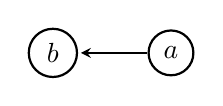
\begin{tikzpicture}[
            > = stealth, % arrow head style
            shorten > = 1pt, % don't touch arrow head to node
            auto,
            node distance = 1.5cm, % distance between nodes
            semithick % line style
        ]

        \tikzstyle{every state}=[
            draw = black,
            thick,
            fill = white,
            minimum size = 4mm
        ]

        \node[state] (b) {$b$};
        \node[state] (a) [right of=b] {$a$};

        \path[->] (a) edge node {} (b);

  \end{tikzpicture}
\end{center}

The third pigeon (shown as pigeon $x$) that needs to be inserted into the row will have one of the four relationships with the two pigeons (shown as $a$ and $b$) in the list:

\begin{center}
  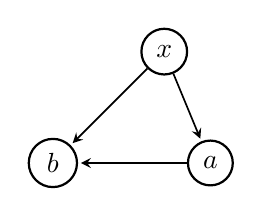
\begin{tikzpicture}[
            > = stealth, % arrow head style
            shorten > = 1pt, % don't touch arrow head to node
            auto,
            node distance = 2cm, % distance between nodes
            semithick % line style
        ]

        \tikzstyle{every state}=[
            draw = black,
            thick,
            fill = white,
            minimum size = 4mm
        ]

        \node[state] (b) {$b$};
        \node[state] (x) [above right of=b] {$x$};
        \node[state] (a) [right of=b] {$a$};

        \path[->] (x) edge node {} (b);
        \path[->] (x) edge node {} (a);
        \path[->] (a) edge node {} (b);

  \end{tikzpicture}
  \qquad
 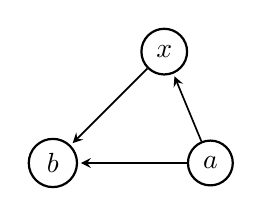
\begin{tikzpicture}[
            > = stealth, % arrow head style
            shorten > = 1pt, % don't touch arrow head to node
            auto,
            node distance = 2cm, % distance between nodes
            semithick % line style
        ]

        \tikzstyle{every state}=[
            draw = black,
            thick,
            fill = white,
            minimum size = 4mm
        ]

        \node[state] (b) {$b$};
        \node[state] (x) [above right of=b] {$x$};
        \node[state] (a) [right of=b] {$a$};

        \path[->] (x) edge node {} (b);
        \path[->] (a) edge node {} (x);
        \path[->] (a) edge node {} (b);

  \end{tikzpicture}
  \qquad
 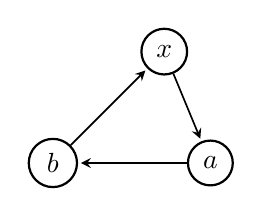
\begin{tikzpicture}[
            > = stealth, % arrow head style
            shorten > = 1pt, % don't touch arrow head to node
            auto,
            node distance = 2cm, % distance between nodes
            semithick % line style
        ]

        \tikzstyle{every state}=[
            draw = black,
            thick,
            fill = white,
            minimum size = 4mm
        ]

        \node[state] (b) {$b$};
        \node[state] (x) [above right of=b] {$x$};
        \node[state] (a) [right of=b] {$a$};

        \path[->] (b) edge node {} (x);
        \path[->] (x) edge node {} (a);
        \path[->] (a) edge node {} (b);

  \end{tikzpicture}
  \qquad
 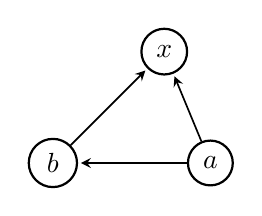
\begin{tikzpicture}[
            > = stealth, % arrow head style
            shorten > = 1pt, % don't touch arrow head to node
            auto,
            node distance = 2cm, % distance between nodes
            semithick % line style
        ]

        \tikzstyle{every state}=[
            draw = black,
            thick,
            fill = white,
            minimum size = 4mm
        ]

        \node[state] (b) {$b$};
        \node[state] (x) [above right of=b] {$x$};
        \node[state] (a) [right of=b] {$a$};

        \path[->] (b) edge node {} (x);
        \path[->] (a) edge node {} (x);
        \path[->] (a) edge node {} (b);

  \end{tikzpicture}
\end{center}

For each of these four cases, the new pigeon can be inserted into the row as shown below.

\begin{center}
  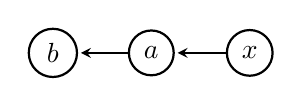
\begin{tikzpicture}[
            > = stealth, % arrow head style
            shorten > = 1pt, % don't touch arrow head to node
            auto,
            node distance = 1.25cm, % distance between nodes
            semithick % line style
        ]

        \tikzstyle{every state}=[
            draw = black,
            thick,
            fill = white,
            minimum size = 4mm
        ]

        \node[state] (b) {$b$};
        \node[state] (a) [right of=b] {$a$};
        \node[state] (x) [right of=a] {$x$};

        \path[->] (a) edge node {} (b);
        \path[->] (x) edge node {} (a);

  \end{tikzpicture}
  \qquad
  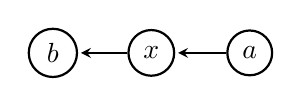
\begin{tikzpicture}[
            > = stealth, % arrow head style
            shorten > = 1pt, % don't touch arrow head to node
            auto,
            node distance = 1.25cm, % distance between nodes
            semithick % line style
        ]

        \tikzstyle{every state}=[
            draw = black,
            thick,
            fill = white,
            minimum size = 4mm
        ]

        \node[state] (b) {$b$};
        \node[state] (x) [right of=b] {$x$};
        \node[state] (a) [right of=x] {$a$};

        \path[->] (x) edge node {} (b);
        \path[->] (a) edge node {} (x);

  \end{tikzpicture}
  \qquad
  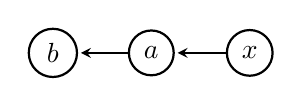
\begin{tikzpicture}[
            > = stealth, % arrow head style
            shorten > = 1pt, % don't touch arrow head to node
            auto,
            node distance = 1.25cm, % distance between nodes
            semithick % line style
        ]

        \tikzstyle{every state}=[
            draw = black,
            thick,
            fill = white,
            minimum size = 4mm
        ]

        \node[state] (b) {$b$};
        \node[state] (a) [right of=b] {$a$};
        \node[state] (x) [right of=a] {$x$};

        \path[->] (a) edge node {} (b);
        \path[->] (x) edge node {} (a);

  \end{tikzpicture}
  \qquad
  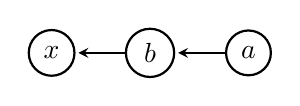
\begin{tikzpicture}[
            > = stealth, % arrow head style
            shorten > = 1pt, % don't touch arrow head to node
            auto,
            node distance = 1.25cm, % distance between nodes
            semithick % line style
        ]

        \tikzstyle{every state}=[
            draw = black,
            thick,
            fill = white,
            minimum size = 4mm
        ]

        \node[state] (x) {$x$};
        \node[state] (b) [right of=x] {$b$};
        \node[state] (a) [right of=b] {$a$};

        \path[->] (a) edge node {} (b);
        \path[->] (b) edge node {} (x);

  \end{tikzpicture}
\end{center}

As a general rule, every pigeon that needs to be inserted into the pecking order list, can be inserted before (to the right of) the first pigeon it pecks, starting from the rightmost pigeon already in the list. Since the newly inserted pigeon pecks the pigeon it is inserted before, it does not violate the rule of the pecking order. If the newly inserted pigeon is inserted before the first pigeon in the list, then we do not have to worry about any pigeon to the right of the insertion point. If the newly inserted pigeon is not inserted before the first pigeon in the list, then it would have been inserted at that point because the pigeon to its right would have pecked it. So again it does not violate the rule of the pecking order

In the case where the pigeon that needs to be inserted into the pecking order list is pecked by every pigeon in the list, the pigeon can be inserted at the end of the list. Again this insertion point does not violate the rule of the pecking order.

So this algorithm is correct.

This is shown below for pigeon $y$ being inserted into a list of three pigeons $a$, $b$ and $c$ and also for a list of four pigeons $a$, $b$, $c$ and $d$. The rule however will hold for any pecking order list size.

\begin{center}
  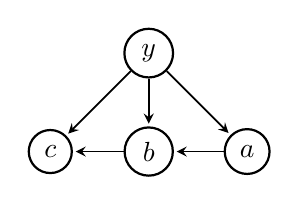
\begin{tikzpicture}[
            > = stealth, % arrow head style
            shorten > = 1pt, % don't touch arrow head to node
            auto,
            node distance = 1.25cm, % distance between nodes
            semithick % line style
        ]

        \tikzstyle{every state}=[
            draw = black,
            thick,
            fill = white,
            minimum size = 4mm
        ]

        \node[state] (b) {$b$};
        \node[state] (y) [above of=b] {$y$};
        \node[state] (a) [right of=b] {$a$};
        \node[state] (c) [left of=b] {$c$};

        \path[->] (y) edge node {} (a);
        \path[->] (y) edge node {} (b);
        \path[->] (y) edge node {} (c);
        \path[->] (a) edge node {} (b);
        \path[->] (b) edge node {} (c);

  \end{tikzpicture}
  \qquad
 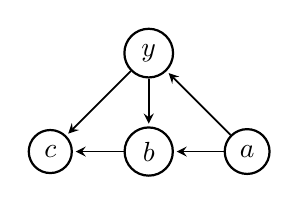
\begin{tikzpicture}[
            > = stealth, % arrow head style
            shorten > = 1pt, % don't touch arrow head to node
            auto,
            node distance = 1.25cm, % distance between nodes
            semithick % line style
        ]

        \tikzstyle{every state}=[
            draw = black,
            thick,
            fill = white,
            minimum size = 4mm
        ]

        \node[state] (b) {$b$};
        \node[state] (y) [above of=b] {$y$};
        \node[state] (a) [right of=b] {$a$};
        \node[state] (c) [left of=b] {$c$};

        \path[->] (a) edge node {} (y);
        \path[->] (y) edge node {} (b);
        \path[->] (y) edge node {} (c);
        \path[->] (a) edge node {} (b);
        \path[->] (b) edge node {} (c);

  \end{tikzpicture}
  \qquad
 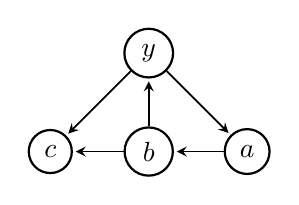
\begin{tikzpicture}[
            > = stealth, % arrow head style
            shorten > = 1pt, % don't touch arrow head to node
            auto,
            node distance = 1.25cm, % distance between nodes
            semithick % line style
        ]

        \tikzstyle{every state}=[
            draw = black,
            thick,
            fill = white,
            minimum size = 4mm
        ]

        \node[state] (b) {$b$};
        \node[state] (y) [above of=b] {$y$};
        \node[state] (a) [right of=b] {$a$};
        \node[state] (c) [left of=b] {$c$};

        \path[->] (y) edge node {} (a);
        \path[->] (b) edge node {} (y);
        \path[->] (y) edge node {} (c);
        \path[->] (a) edge node {} (b);
        \path[->] (b) edge node {} (c);

  \end{tikzpicture}
  \qquad
 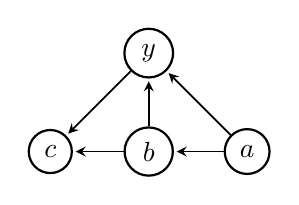
\begin{tikzpicture}[
            > = stealth, % arrow head style
            shorten > = 1pt, % don't touch arrow head to node
            auto,
            node distance = 1.25cm, % distance between nodes
            semithick % line style
        ]

        \tikzstyle{every state}=[
            draw = black,
            thick,
            fill = white,
            minimum size = 4mm
        ]

        \node[state] (b) {$b$};
        \node[state] (y) [above of=b] {$y$};
        \node[state] (a) [right of=b] {$a$};
        \node[state] (c) [left of=b] {$c$};

        \path[->] (a) edge node {} (y);
        \path[->] (b) edge node {} (y);
        \path[->] (y) edge node {} (c);
        \path[->] (a) edge node {} (b);
        \path[->] (b) edge node {} (c);

  \end{tikzpicture}
\end{center}


\begin{center}
  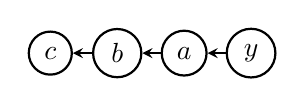
\begin{tikzpicture}[
            > = stealth, % arrow head style
            auto,
            node distance = 0.85cm, % distance between nodes
            semithick % line style
        ]

        \tikzstyle{every state}=[
            draw = black,
            thick,
            fill = white,
            minimum size = 4mm
        ]

        \node[state] (b) {$b$};
        \node[state] (a) [right of=b] {$a$};
        \node[state] (c) [left of=b] {$c$};
        \node[state] (y) [right of=a] {$y$};

        \path[->] (a) edge node {} (b);
        \path[->] (b) edge node {} (c);
        \path[->] (y) edge node {} (a);

  \end{tikzpicture}
  \qquad
  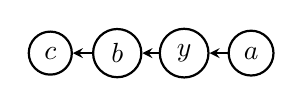
\begin{tikzpicture}[
            > = stealth, % arrow head style
            auto,
            node distance = 0.85cm, % distance between nodes
            semithick % line style
        ]

        \tikzstyle{every state}=[
            draw = black,
            thick,
            fill = white,
            minimum size = 4mm
        ]

        \node[state] (b) {$b$};
        \node[state] (y) [right of=b] {$y$};
        \node[state] (c) [left of=b] {$c$};
        \node[state] (a) [right of=y] {$a$};

        \path[->] (y) edge node {} (b);
        \path[->] (b) edge node {} (c);
        \path[->] (a) edge node {} (y);

  \end{tikzpicture}
  \qquad
  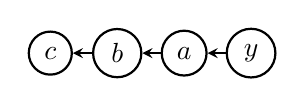
\begin{tikzpicture}[
            > = stealth, % arrow head style
            auto,
            node distance = 0.85cm, % distance between nodes
            semithick % line style
        ]

        \tikzstyle{every state}=[
            draw = black,
            thick,
            fill = white,
            minimum size = 4mm
        ]

        \node[state] (b) {$b$};
        \node[state] (a) [right of=b] {$a$};
        \node[state] (c) [left of=b] {$c$};
        \node[state] (y) [right of=a] {$y$};

        \path[->] (a) edge node {} (b);
        \path[->] (b) edge node {} (c);
        \path[->] (y) edge node {} (a);

  \end{tikzpicture}
  \qquad
  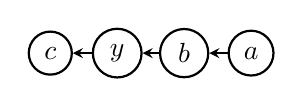
\begin{tikzpicture}[
            > = stealth, % arrow head style
            auto,
            node distance = 0.85cm, % distance between nodes
            semithick % line style
        ]

        \tikzstyle{every state}=[
            draw = black,
            thick,
            fill = white,
            minimum size = 4mm
        ]

        \node[state] (b) {$b$};
        \node[state] (a) [right of=b] {$a$};
        \node[state] (y) [left of=b] {$y$};
        \node[state] (c) [left of=y] {$c$};

        \path[->] (a) edge node {} (b);
        \path[->] (b) edge node {} (y);
        \path[->] (y) edge node {} (c);

  \end{tikzpicture}
\end{center}

\begin{center}
  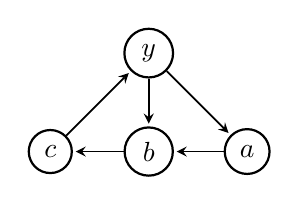
\begin{tikzpicture}[
            > = stealth, % arrow head style
            shorten > = 1pt, % don't touch arrow head to node
            auto,
            node distance = 1.25cm, % distance between nodes
            semithick % line style
        ]

        \tikzstyle{every state}=[
            draw = black,
            thick,
            fill = white,
            minimum size = 4mm
        ]

        \node[state] (b) {$b$};
        \node[state] (y) [above of=b] {$y$};
        \node[state] (a) [right of=b] {$a$};
        \node[state] (c) [left of=b] {$c$};

        \path[->] (y) edge node {} (a);
        \path[->] (y) edge node {} (b);
        \path[->] (c) edge node {} (y);
        \path[->] (a) edge node {} (b);
        \path[->] (b) edge node {} (c);

  \end{tikzpicture}
  \qquad
 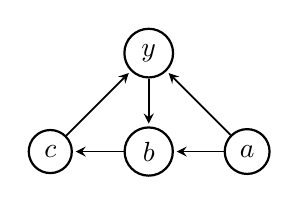
\begin{tikzpicture}[
            > = stealth, % arrow head style
            shorten > = 1pt, % don't touch arrow head to node
            auto,
            node distance = 1.25cm, % distance between nodes
            semithick % line style
        ]

        \tikzstyle{every state}=[
            draw = black,
            thick,
            fill = white,
            minimum size = 4mm
        ]

        \node[state] (b) {$b$};
        \node[state] (y) [above of=b] {$y$};
        \node[state] (a) [right of=b] {$a$};
        \node[state] (c) [left of=b] {$c$};

        \path[->] (a) edge node {} (y);
        \path[->] (y) edge node {} (b);
        \path[->] (c) edge node {} (y);
        \path[->] (a) edge node {} (b);
        \path[->] (b) edge node {} (c);

  \end{tikzpicture}
  \qquad
 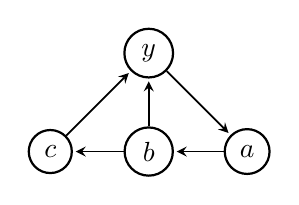
\begin{tikzpicture}[
            > = stealth, % arrow head style
            shorten > = 1pt, % don't touch arrow head to node
            auto,
            node distance = 1.25cm, % distance between nodes
            semithick % line style
        ]

        \tikzstyle{every state}=[
            draw = black,
            thick,
            fill = white,
            minimum size = 4mm
        ]

        \node[state] (b) {$b$};
        \node[state] (y) [above of=b] {$y$};
        \node[state] (a) [right of=b] {$a$};
        \node[state] (c) [left of=b] {$c$};

        \path[->] (y) edge node {} (a);
        \path[->] (b) edge node {} (y);
        \path[->] (c) edge node {} (y);
        \path[->] (a) edge node {} (b);
        \path[->] (b) edge node {} (c);

  \end{tikzpicture}
\end{center}


\begin{center}
  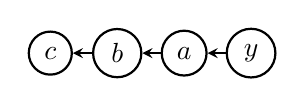
\begin{tikzpicture}[
            > = stealth, % arrow head style
            auto,
            node distance = 0.85cm, % distance between nodes
            semithick % line style
        ]

        \tikzstyle{every state}=[
            draw = black,
            thick,
            fill = white,
            minimum size = 4mm
        ]

        \node[state] (b) {$b$};
        \node[state] (a) [right of=b] {$a$};
        \node[state] (c) [left of=b] {$c$};
        \node[state] (y) [right of=a] {$y$};

        \path[->] (a) edge node {} (b);
        \path[->] (b) edge node {} (c);
        \path[->] (y) edge node {} (a);

  \end{tikzpicture}
  \qquad
  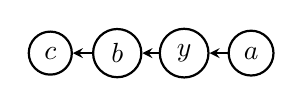
\begin{tikzpicture}[
            > = stealth, % arrow head style
            auto,
            node distance = 0.85cm, % distance between nodes
            semithick % line style
        ]

        \tikzstyle{every state}=[
            draw = black,
            thick,
            fill = white,
            minimum size = 4mm
        ]

        \node[state] (b) {$b$};
        \node[state] (y) [right of=b] {$y$};
        \node[state] (c) [left of=b] {$c$};
        \node[state] (a) [right of=y] {$a$};

        \path[->] (y) edge node {} (b);
        \path[->] (b) edge node {} (c);
        \path[->] (a) edge node {} (y);

  \end{tikzpicture}
  \qquad
  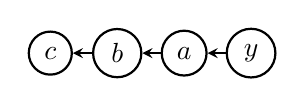
\begin{tikzpicture}[
            > = stealth, % arrow head style
            auto,
            node distance = 0.85cm, % distance between nodes
            semithick % line style
        ]

        \tikzstyle{every state}=[
            draw = black,
            thick,
            fill = white,
            minimum size = 4mm
        ]

        \node[state] (b) {$b$};
        \node[state] (a) [right of=b] {$a$};
        \node[state] (c) [left of=b] {$c$};
        \node[state] (y) [right of=a] {$y$};

        \path[->] (a) edge node {} (b);
        \path[->] (b) edge node {} (c);
        \path[->] (y) edge node {} (a);

  \end{tikzpicture}
\end{center}

\begin{center}
  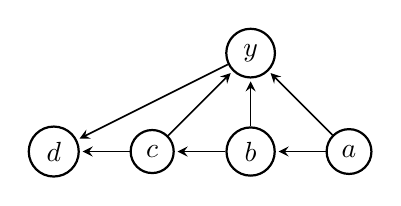
\begin{tikzpicture}[
            > = stealth, % arrow head style
            shorten > = 1pt, % don't touch arrow head to node
            auto,
            node distance = 1.25cm, % distance between nodes
            semithick % line style
        ]

        \tikzstyle{every state}=[
            draw = black,
            thick,
            fill = white,
            minimum size = 4mm
        ]

        \node[state] (b) {$b$};
        \node[state] (y) [above of=b] {$y$};
        \node[state] (a) [right of=b] {$a$};
        \node[state] (c) [left of=b] {$c$};
        \node[state] (d) [left of=c] {$d$};

        \path[->] (a) edge node {} (y);
        \path[->] (b) edge node {} (y);
        \path[->] (c) edge node {} (y);
        \path[->] (a) edge node {} (b);
        \path[->] (b) edge node {} (c);
        \path[->] (c) edge node {} (d);
        \path[->] (y) edge node {} (d);

  \end{tikzpicture}
  \qquad
 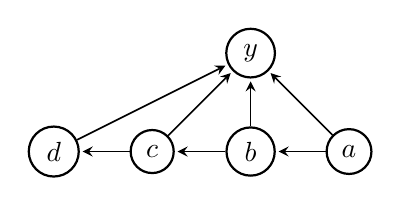
\begin{tikzpicture}[
            > = stealth, % arrow head style
            shorten > = 1pt, % don't touch arrow head to node
            auto,
            node distance = 1.25cm, % distance between nodes
            semithick % line style
        ]

        \tikzstyle{every state}=[
            draw = black,
            thick,
            fill = white,
            minimum size = 4mm
        ]

        \node[state] (b) {$b$};
        \node[state] (y) [above of=b] {$y$};
        \node[state] (a) [right of=b] {$a$};
        \node[state] (c) [left of=b] {$c$};
        \node[state] (d) [left of=c] {$d$};

        \path[->] (a) edge node {} (y);
        \path[->] (b) edge node {} (y);
        \path[->] (c) edge node {} (y);
        \path[->] (a) edge node {} (b);
        \path[->] (b) edge node {} (c);
        \path[->] (c) edge node {} (d);
        \path[->] (d) edge node {} (y);

  \end{tikzpicture}
\end{center}


\begin{center}
  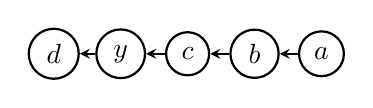
\begin{tikzpicture}[
            > = stealth, % arrow head style
            auto,
            node distance = 0.85cm, % distance between nodes
            semithick % line style
        ]

        \tikzstyle{every state}=[
            draw = black,
            thick,
            fill = white,
            minimum size = 4mm
        ]

        \node[state] (b) {$b$};
        \node[state] (a) [right of=b] {$a$};
        \node[state] (c) [left of=b] {$c$};
        \node[state] (y) [left of=c] {$y$};
        \node[state] (d) [left of=y] {$d$};

        \path[->] (a) edge node {} (b);
        \path[->] (b) edge node {} (c);
        \path[->] (c) edge node {} (y);
        \path[->] (y) edge node {} (d);

  \end{tikzpicture}
  \qquad
  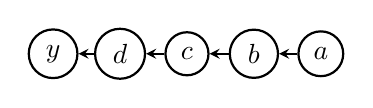
\begin{tikzpicture}[
            > = stealth, % arrow head style
            auto,
            node distance = 0.85cm, % distance between nodes
            semithick % line style
        ]

        \tikzstyle{every state}=[
            draw = black,
            thick,
            fill = white,
            minimum size = 4mm
        ]

        \node[state] (b) {$b$};
        \node[state] (a) [right of=b] {$a$};
        \node[state] (c) [left of=b] {$c$};
        \node[state] (d) [left of=c] {$d$};
        \node[state] (y) [left of=d] {$y$};

        \path[->] (a) edge node {} (b);
        \path[->] (b) edge node {} (c);
        \path[->] (c) edge node {} (d);
        \path[->] (d) edge node {} (y);

  \end{tikzpicture}
\end{center}

\part We can assume that the directed graph is stored as an adjacency list with every node for a pigeon containing a list of other pigeons it pecks. This list does not have to be sorted. The pecking order for the pigeons can be stored as a linked list with the pigeon being pecked pointed to by the pecking pigeon. Here is the algorithm for a pecking order list for the pigeons.

\let\oldReturn\Return
\renewcommand{\Return}{\State\oldReturn}

\begin{minipage}{\linewidth}
  \begin{algorithm}[H]
    \caption{Pecking Order List Algorithm}\label{AlgPeck}
    \begin{algorithmic}[1]
      \Procedure{PeckingOrderListAlgorithm}{Pecking Order Relationship Graph}
      	\State Create empty Pecking Order List
	\While {there are more nodes in directed graph}
		\State Get next node
		\If {pecking order list is empty}
			\State Add new node to the list
		\Else
			\State Look for first node in list pecked by new node
			\If {found}
				\State Insert new node to the right of the pecked node found
			\Else
				\State Insert new node at the left end of the list
			\EndIf
		\EndIf
	\EndWhile
	\Return Pecking Order List
      \EndProcedure
    \end{algorithmic}
  \end{algorithm}
\end{minipage}\\\\

\end{parts}

\textbf{Analysys of algorithm time complexity:}
Let $n$ be the total number of pigeons. The $while$ loop will execute $n$ times. The worst case for the step of looking for the first node in the list that is pecked by the new node will look through every node in the list. This will go through $1$ node the first time around, $2$ nodes the second time around and $n-1$ nodes when the last new node is added. So this step will take a total of $O(n^2)$ time. Every other step will take constant time. So the entire algorithm will run in $O(n^2)$ time.

\color{qcolor}
\titledquestion{More divide, better run time}
{\em Moral:} as long as the ``conquer'' step is not too expensive, dividing a problem into smaller sub-problems typically helps. 

Consider the problem of multiplying two $n$-digit integers.  We saw in class (Lecture 3, Karatsuba's algorithm) that dividing into two $n/2$ bit numbers and combining appropriately, we can compute the product in time $O(n^{1.585..})$. So we can wonder: can division into three pieces help?

Suppose we have two $n$-digit integers $A, B$. Split $A$ into $A_1$,  $A_2$ and $A_3$, each having $n/3$ digits (assume $n$ is a power of $3$ for this problem). So also, split $B$ into $B_1, B_2$ and $B_3$. If the numbers are in base 10, we can write $A = 10^{2n/3} A_1 + 10^{n/3} A_2 + A_3$.  Let $p(z)$ be the polynomial $A_1 z^2 + A_2 z + A_3$, and let $q(z) = B_1 z^2 + B_2 z + B_3$.  Define $r(z) = p(z) q(z)$.  The degree of $r(z)$ is $4$, so $r(z) = C_1 z^4 + C_2 z^3 + C_3 z^2 + C_4 z + C_5$, for some coefficients $C_i$.  

\begin{parts}
\part[2] Observe that the product of $A$ and $B$ is $r(10^{n/3})$.
\part[2] Observe that once we know the $C_i$, assuming they are $O(n)$ digits each, $r(10^{n/3})$ can be found in $O(n)$ time.
\part[4] We thus need to find the $C_i$. The trick is to find the values of $r(z)$ at a few {\em small} values of $z$. Specifically, we find $r(z)$ for $z \in \{-2, -1, 0, 1, 2\}$. Show that we can compute each of these $r(z)$ in time $T(n/3) + O(n)$, where $T(n/3)$ is the time needed to multiply two $n/3$ digit numbers.  Explain why these values uniquely determine $C_i$.  [{\em Hint:} use $ r = p \cdot q$, and the degree of $r$.]
\part[4] To find the $C_i$, write a system of linear equations, and show how these can be solved to obtain $C_i$ in $O(n)$ time.

These observations let us conclude that $T(n) = 5 T(n/3) + O(n)$, which results in an overall run time of $O(n^{1.464..})$, which is better than Karatsuba's algorithm. (This can be pushed further, to obtain $n^{1+\epsilon}$, for any constant $\epsilon >0$.)
\end{parts}

\color{acolor}

\begin{parts}

\part \begin{equation*}
\begin{aligned}
A &= 10^{\frac{2n}{3}} A_1 + 10^{\frac{n}{3}} A_2 +  A_3\\\
&= A_1 z^2 + A_2 z +  A_3 \text{, when $z=10^{\frac{n}{3}}$}\\
B &= 10^{\frac{2n}{3}} B_1 + 10^{\frac{n}{3}} B_2 + B_3\\
&= B_1 z^2 + B_2 z +  B_3 \text{, when $z=10^{\frac{n}{3}}$}\\
\Rightarrow A \times B &= p(z)q(z) \text{, when $z=10^{\frac{n}{3}}$}\\
&= r(z) \text{, when $z=10^{\frac{n}{3}}$}\\
&= r(10^{n/3})
\end{aligned}
\end{equation*}

\part Once we know each $C_i$, if each of these is $O(n)$ digits each, we can find $r(10^{n/3})$ by shifting each $C_i$ to the left by $\frac{n}{3}$ times the power of the associated $z$ term and then adding all the terms. The total amount of work involved in shifting will be $ \frac{n}{3} + \frac{2n}{3} + \frac{3n}{3} + \frac{4n}{3} = \frac{10n}{3}$. The work of adding the $5$ terms will be $4\times\frac{5n}{3}$, since we need to add $5$ numbers the longest of which is $\frac{5n}{3}$ digits. So the total time for finding $r(10^{n/3})$ will be $O(n)$.

\part \begin{equation*}
\begin{aligned}
r(2) =p(2)q(2)=(4A1+2A2+A3)(4B1+2B2+B3)
\end{aligned}
\end{equation*}
$r(1)$, $r(0)$, $r(-1)$ and $r(-2)$ can be written out similarly. 4 times a binary number is just the number shifted left two times and 2 times a binary number is just the number shifted left once. The additions before multiplying the two terms in each $r(z)$ can be done in $O(n)$ time. Then we would need to multiply two $n/3$ digit numbers. There may be an extra digit due to the multiplication by $4$, $2$ or because of the addition. However on the average, each $r(z)$ can be computed in time $T(n/3) + O(n)$, where $T(n/3)$ is the time needed to multiply two $n/3$ digit numbers.

Once we find the $r(z)$ vales for $z \in \{-2, -1, 0, 1, 2\}$, we can construct $5$ equations in the $C_i$'s. For example, corresponding to $z=2$, we have the following equation:
$$
16C_1 + 8C_2+4C_3+2C_4+C_5 = r(2)
$$
Since we will have a total of $5$ $r(z)$ values, we can construct $5$ equations of the form shown above in the $5$ $C_i$ variables. This will enable us to solve the $5$ equations in $5$ variables to uniquely determine the $C_i$ values.

\part \begin{equation*}
\begin{aligned}
16C_1 + 8C_2+4C_3+2C_4+C_5 &= r(2)\\
C_1 + C_2+C_3+C_4+C_5&= r(1)\\
C_5&= r(0)\\
C_1 -C_2+C_3-C_4+C_5&= r(-1)\\
16C_1 - 8C_2+4C_3-2C_4+C_5 &= r(-2)
\end{aligned}
\end{equation*}

If we add the first and last equations, we get one equation in $C_1$ and $C_3$ since $C_2$ and $C_4$ get eliminated and $C_5$ is given by the third equation. We can get another equation in $C_1$ and $C_3$ by adding the second and fourth equations. Each of these steps will take $O(n)$ time. We can now solve two equations in $C_1$ and $C_3$ by subtracting the equations after multiplying them by the relevant constant. Once we know $C_1$ and $C_3$, we can get two equations in $C_2$ and $C_4$ with can also similarly solved in $O(n)$ time. So the equations can be solved to obtain $C_i$ in $O(n)$ time.

These observations above lead us to conclude that two $n$ digit numbers can be multiplied in $T(n) = 5 \times \text{time for each $r(z)$} + \text{$O(n)$ time for solving each $C_i$} =5 T(n/3) + O(n)$ time.

According to the Master Theorem, $a=5$, $b=3$ and $\log_b a = \log_3 5 = 1.464..$. Since $f(n) = O(n)$, this corresponds to case 1 of the Master Theorem and so $T(n) = \Theta(n^{1.464..})$, or  $T(n) =O(n^{1.464..})$.

\end{parts}

\end{questions}

\begin{thebibliography}{9}

\bibitem{CLRS} \enquote{4.5 The master method for solving recurrences.} \textit{Introduction to Algorithms}, by Thomas H. Cormen et al., Mit Press, 2009, pp. 94-94.

\end{thebibliography}

\end{document}
